\documentclass[aps,prresearch,reprint,superscriptaddress,floatfix,amsmath,amssymb]{revtex4-2}

\usepackage{graphicx}
\usepackage{booktabs}
\usepackage{bm}
\usepackage{mathtools}
\usepackage{xr-hyper}
\usepackage{hyperref}
\usepackage{orcidlink}
\hypersetup{hidelinks}
\externaldocument[M-][nocite]{main}

\newcommand{\dd}{\mathrm{d}}
\newcommand{\ee}{\mathrm{e}}
\newcommand{\ii}{\mathrm{i}}
\newcommand{\Ree}{\operatorname{Re}}
\newcommand{\Imm}{\operatorname{Im}}
\newcommand{\Tr}{\operatorname{Tr}}
\newcommand{\I}{\mathcal{I}}

\begin{document}

\title{Supplemental Material for ``Exceptional-point unfolding and critical
bare-energy return in a frequency-swept qubit''}

\author{Francisco Ahumada}
\affiliation{Departamento de F\'isica, Universidad T\'ecnica Federico Santa Mar\'ia,
Casilla 110-V, Valpara\'iso, Chile}
\author{Felipe Barra}
\affiliation{Departamento de F\'isica, Facultad de Ciencias F\'isicas y
Matem\'aticas, Universidad de Chile, 837.0415 Santiago, Chile}
\author{Ariel Norambuena\orcidlink{0000-0001-9496-8765}}
\email{ariel.norambuena@usm.cl}
\affiliation{Departamento de F\'isica, Universidad T\'ecnica Federico Santa Mar\'ia,
Casilla 110-V, Valpara\'iso, Chile}

\date{July 17, 2026}
\maketitle

\setcounter{equation}{0}
\renewcommand{\theequation}{S\arabic{equation}}
\setcounter{figure}{0}
\renewcommand{\thefigure}{S\arabic{figure}}
\setcounter{table}{0}
\renewcommand{\thetable}{S\Roman{table}}

This Supplemental Material contains the analytical extensions, numerical
certifications, and microscopic reconstructions supporting the focused main
article. References to equations and figures without an ``S'' prefix refer
to the main article.



\section{Exceptional-point critical layer}
\label{sec:s_critical_layer}

This section gives the perturbative details suppressed from the main text.
For the linear representative \(\delta=a\tau\),
Eq.~\eqref{M-eq:generalDetuningDynamics} reads
\begin{equation}
u''+\left[
\frac{\ell(2-\ell)}4+\frac{a^2\tau^2}{4}
-\frac{\ii a}{2}-\frac{\ii\ell a\tau}{2}
\right]u=0.
\label{eq:s_linear_gauge}
\end{equation}
Introduce
\begin{equation}
\epsilon=a^{1/4},\qquad
2-\ell=\mu\epsilon^2,\qquad
s=\epsilon\tau,\qquad
U(s)=\epsilon u(\tau).
\label{eq:s_critical_scaling}
\end{equation}
The transformed initial data are \(U(0)=\epsilon\) and
\(U'(0)=\ell/2\). Equation~\eqref{eq:s_linear_gauge} becomes
\begin{equation}
U''+\left[
\frac{\mu}{2}-\frac{\ii\ell\epsilon s}{2}
-\epsilon^2\left(\frac{\mu^2}{4}+\frac{\ii}{2}\right)
+\frac{\epsilon^4s^2}{4}
\right]U=0.
\label{eq:s_scaled_critical}
\end{equation}
With
\(\mu=\mu_0+\epsilon\mu_1+\epsilon^2\mu_2+\cdots\) and
\(U=U_0+\epsilon U_1+\epsilon^2U_2+\cdots\), define
\(\mathcal L=\dd^2/\dd s^2+k^2\), \(k^2=\mu_0/2\). The first three
orders are
\begin{align}
\mathcal L U_0&=0,
\label{eq:U0hierarchy}\\
\mathcal L U_1&=\left(\ii s-\frac{\mu_1}{2}\right)U_0,
\label{eq:U1hierarchy}\\
\mathcal L U_2&=\left(\ii s-\frac{\mu_1}{2}\right)U_1
+\left(\frac{\mu_0^2}{4}+\frac{\ii}{2}
-\frac{\mu_2}{2}\right)U_0.
\label{eq:U2hierarchy}
\end{align}
The leading initial conditions give
\begin{equation}
U_0(s)=\frac{\sin(ks)}{k}.
\label{eq:Uzero}
\end{equation}
The inverse of \(\mathcal L\) with zero initial data is the retarded Green
function
\begin{equation}
\begin{aligned}
G(s,r)&=\frac{\sin[k(s-r)]}{k}\Theta(s-r),\\
(\mathcal L^{-1}F)(s)&=\int_0^sG(s,r)F(r)\dd r.
\end{aligned}
\label{eq:criticalGreenfunction}
\end{equation}
At the first zero \(s_0=\pi/k\), the chirp-induced imaginary lift is
\begin{equation}
w_0=\frac1{k^2}\int_0^{\pi/k}r\sin^2(kr)\dd r
=\frac{\pi^2}{4k^4}.
\label{eq:s_wzero}
\end{equation}
Writing \(s=s_0+\epsilon\xi\) gives
\(\Ree q=-1+v/(v^2+w_0^2)+O(\epsilon)\), with \(v=\xi+1\).
The maximum occurs at \(v=w_0\); double tangency therefore requires
\(w_0=1/2\), yielding \(\mu_0=\sqrt2\pi\).

To obtain the next coefficient, solve Eq.~\eqref{eq:U1hierarchy} as
\begin{align}
U_1&=\cos(ks)+\ii w(s)-\frac{\mu_1}{2}z(s),\nonumber\\
z(s)&=-\frac{s\cos(ks)}{2k^2}
+\frac{\sin(ks)}{2k^3},
\label{eq:zfunction}
\end{align}
where the cosine enforces \(U_1(0)=1\), and
\begin{equation}
\begin{aligned}
w(s)&=\int_0^sG(s,r)rU_0(r)\dd r,\\
z(s)&=\int_0^sG(s,r)U_0(r)\dd r.
\end{aligned}
\label{eq:wzGreen}
\end{equation}
Thus ``Green-function integral'' means the exact inverse of the
constant-coefficient operator \(\mathcal L\), not an additional
approximation. At \(s_0\),
\begin{equation}
d:=w'(s_0)=\frac{\pi}{4k^3},
\qquad z(s_0)=\frac{\pi}{2k^3},
\qquad z'(s_0)=0.
\label{eq:criticalvalues}
\end{equation}
If \(v_2=\Imm U_2\), the only second-order value entering the tangency is
\begin{equation}
v_2(s_0)=\mu_1A_1,
\qquad A_1=-\frac{3\pi^2}{16k^6}.
\label{eq:A1}
\end{equation}
Indeed, Eq.~\eqref{eq:U2hierarchy} has the exact representation
\begin{equation}
U_2(s)=U_2^{\rm hom}(s)+\int_0^sG(s,r)\mathcal S_2(r)\dd r,
\label{eq:U2Green}
\end{equation}
with \(\mathcal S_2\) equal to the right-hand side of
Eq.~\eqref{eq:U2hierarchy}. Elementary sine integrals then reduce its
imaginary part at \(s_0\) to Eq.~\eqref{eq:A1}; the homogeneous term enforces
the second-order initial derivative and vanishes at \(s_0\). After absorbing
the real displacement into the inner coordinate,
\begin{equation}
\max_\xi\Ree q=
2\epsilon\left[d+\mu_1(d^2-A_1)\right]+O(\epsilon^2).
\label{eq:qnext}
\end{equation}
The tangency condition gives
\begin{equation}
\mu_1=\frac{d}{A_1-d^2}
=-\frac{k^3}{\pi}
=-\frac{\sqrt\pi}{2^{3/4}},
\label{eq:s_mu1}
\end{equation}
which proves the second fractional coefficient in
Eq.~\eqref{M-eq:mainboundary} without fitting.


\section{Control-profile robustness}
\label{subsec:profileuniversality}

The first two fractional coefficients are not restricted to an exactly linear
waveform. To separate the local passage through resonance from the arbitrary
late-time shape of the control, we introduce a dimensionless profile \(f\)
and generate a one-parameter slow family by changing only its time scale:
\begin{align}
\delta_a(\tau)&=d f(a\tau/d),\nonumber\\
f(x)&=x+c_mx^m+O(x^{m+1}),\quad m\geq2,
\label{eq:profilefamily}
\end{align}
Here, \(d\) fixes the eventual detuning scale and every member has the same
initial slope \(\delta_a'(0)=a\). This construction includes linear ramps on
a finite window and bounded protocols such as hyperbolic, arctangent, and
exponential saturations. It is not an assertion that one Taylor series
represents every waveform globally. Rather, it tests which part of the
critical boundary depends only on the local Taylor jet sampled in the
critical layer \(\tau=O(a^{-1/4})\), while the monotone continuation, bounded
first three derivatives, and positive saturation exclude an independently
generated later revival. If the first tangency defines the upper boundary,
perturbation of that layer gives
\begin{align}
\ell_c^{(f)}(a)-\ell_c^{\rm lin}(a)
&=-K_m\frac{c_m}{d^{m-1}}a^{(3m-1)/4}\nonumber\\
&\quad+o\!\left(a^{(3m-1)/4}\right),
\label{eq:profiletheorem}
\end{align}
where
\begin{equation}
K_m=\frac{\mu_0}{k_0^{m+3}}
\int_0^\pi x^m\sin^2x\dd x,
\qquad k_0^2=\frac{\pi}{\sqrt2}.
\label{eq:Km}
\end{equation}
Hence the \(a^{1/2}\) and \(a^{3/4}\) terms are universal among analytic
profiles with the same local slope. A quadratic curvature first enters at
\(a^{5/4}\), whereas an odd profile has its first correction at \(a^2\), with
\(K_3=(\pi^2-3)/2\). Figure~\ref{fig:profileuniversality} verifies the
parameter-free coefficients using \(\tanh x\), \(\arctan x\),
\(x/\sqrt{1+x^2}\), a cubic polynomial, and \(1-\ee^{-x}\).

\begin{figure*}[t]
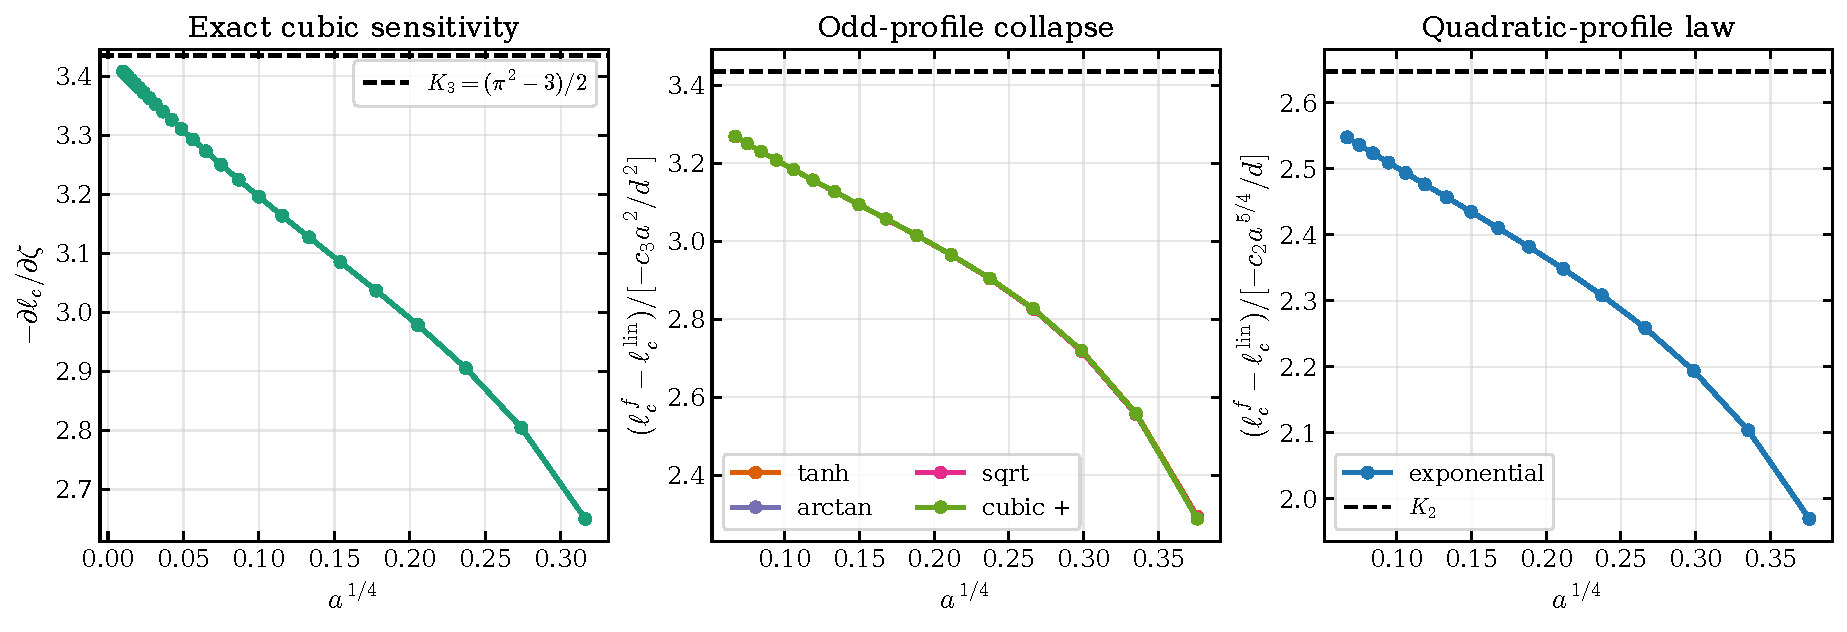
\includegraphics[width=\textwidth]{detuning_universality_theorem.pdf}
\caption{Universality with respect to the control profile. Variational and
direct calculations converge to the analytical constants in
Eqs.~\eqref{eq:profiletheorem} and \eqref{eq:Km}; no fitted critical exponent
is used.}
\label{fig:profileuniversality}
\end{figure*}


\section{Uniform crossover and late-time sign control}
\label{app:uniform}

We now close the gap between the first lifted zero and the full slow
protocol. Let \(\delta_a(\tau)=d f(a\tau/d)\), where
\(f\in C^3([0,\infty))\), \(f(0)=0\), \(f'(0)=1\), \(f'\geq0\), the
first three derivatives are bounded, and \(f\) approaches a positive
constant. Assume \((2-\ell)/\epsilon^2\to\mu_0\), with
\(\epsilon=a^{1/4}\).

Fix \(L>L_0\), independent of \(\epsilon\), and define
\begin{equation}
\begin{aligned}
S_\epsilon&=L\epsilon^{-1/2}\sqrt{\ln(1/\epsilon)},\\
N_\epsilon&=\lfloor\epsilon^{-1/4}\rfloor,
&k_\epsilon^2&=\frac{2-\ell}{2\epsilon^2}.
\end{aligned}
\label{eq:splitindices}
\end{equation}
Then \(k_\epsilon\to k_0\), with
\(k_0^2=\mu_0/2=\pi/\sqrt2\). The constant \(L_0\) is chosen once so that
the Liouville--Green damping accumulated by \(S_\epsilon\) dominates the
algebraic matching errors; it does not grow as \(\epsilon\to0\). There are
\(C,\epsilon_0>0\), independent of the oscillation-cell index, such that
for \(0<\epsilon<\epsilon_0\),
\begin{align}
\sup_{\mathcal C_n}\Ree q
&=-1+\frac1{n^2}+O(\epsilon^{1/2}),
&&2\leq n\leq N_\epsilon,
\label{eq:appendixearly}\\
\sup_{\mathcal C_n}\Ree q
&\leq-1+C\epsilon^{1/2}\ln^{3/2}(1/\epsilon),
&&N_\epsilon\leq n\leq k_0S_\epsilon/\pi.
\label{eq:appendixlate}
\end{align}
In particular, all later cells have a common negative limiting margin.

On the crossover interval the scaled equation has coefficient
\begin{equation}
\begin{aligned}
Q_\epsilon(s)&=k_\epsilon^2-\frac{\ii\ell\epsilon s}{2}
+R_\epsilon(s),\\
|R_\epsilon|+(1+s)^{-1}|R_\epsilon'|
&\leq C\epsilon^2(1+s^2).
\end{aligned}
\label{eq:Qremainder}
\end{equation}
For \(n\leq N_\epsilon\), Duhamel's formula about
\(U_0=\sin(k_\epsilon s)/k_\epsilon\) resolves each lifted zero. Its
imaginary displacement is \(O(\epsilon n^2)\), as is the controlled
remainder after division by the local solution, which proves
Eq.~\eqref{eq:appendixearly}.

For \(n\geq N_\epsilon\), let \(p_a=\sqrt{Q_\epsilon}\), using the branch
continued from \(p_a(0)>0\). The imaginary control term keeps
\(Q_\epsilon\) away from zero on the real crossover, so no turning-point
connection formula is needed. Substitution of
\(p_a^{-1/2}\exp(\pm\ii\int p_a\dd s)\) leaves the standard
Liouville--Green residual
\begin{equation}
\begin{aligned}
\mathcal R_a
&=\frac{3(p_a')^2}{4p_a^3}-\frac{p_a''}{2p_a^2},\\
\int_0^{S_\epsilon}|\mathcal R_a(s)|\dd s
&=O\!\left(\epsilon^{3/2}\sqrt{\ln(1/\epsilon)}\right).
\end{aligned}
\label{eq:LGresidual}
\end{equation}
Variation of constants around this basis is therefore uniform over the
growing number of cells. The accumulated imaginary phase is already
\(O(\epsilon^{1/2})\) at the late-cell entry, preventing a small-denominator
loss and proving Eq.~\eqref{eq:appendixlate}. At the crossover exit,
\begin{equation}
\tau_m=\frac{S_\epsilon}{\epsilon},
\qquad
r_m:=|q(\tau_m)-q_s[\delta_a(\tau_m)]|\leq C\epsilon^2,
\label{eq:entrybound}
\end{equation}
where \(q_s\) is the attracting frozen root of the Riccati equation.

For the remaining tail, write \(e=q-q_s(\delta)\) and
\(\Delta=\sqrt{(\ell+\ii\delta)^2-2\ell}=u+\ii v\), \(u>0\). The exact
Riccati equation gives
\(e'=-\Delta e-e^2-q_{s,\delta}\delta'\). Hence, for \(r=|e|\),
\begin{equation}
D^+r\leq-u r+r^2+|q_{s,\delta}\delta'|.
\label{eq:tubeinequality}
\end{equation}
Let \(u_*\) and \(m_*\) be the minimum of \(u\) and \(-\Ree q_s\) on the
tail, and let \(F_*\) be the maximum forcing. If \(u_*^2>4F_*\), set
\(R_\pm=[u_*\pm\sqrt{u_*^2-4F_*}]/2\). The comparison principle gives
the invariant-tube criterion
\begin{equation}
\max\{r_m,R_-\}<\min\{m_*,R_+\}
\quad\Longrightarrow\quad
\Ree q(\tau)<0
\label{eq:tubecriterion}
\end{equation}
for all later times. Equation~\eqref{eq:entrybound} satisfies this criterion
for sufficiently small \(a\), completing the global sign proof used in the
main text.


\section{Dependence on the finite sweep range}

The three events are not peculiar to a single sweep range, but their order is
range dependent. Table~\ref{tab:rangedependence} continues the exact endpoint
and switch conditions for four values of \(\Omega_\Delta\). All listed
residuals are below \(10^{-10}\).
\begin{table*}[t]
\caption{Dependence of the finite-duration geometry on the detuning range.
The columns give the interior-to-endpoint switch, the weak-coupling endpoint
birth, and the cusp tip.}
\label{tab:rangedependence}
\begin{ruledtabular}
\begin{tabular}{cccccc}
\(\Omega_\Delta\) & \(\ell_{\rm sw}\) & \(a_{\rm sw}\) & \(a_0\) &
\(\ell_t\) & \(a_t\)\\
\hline
1.00 & 0.90056294 & 0.23502958 & 0.21763358 & 0.53649633 & 0.28046829\\
1.25 & 0.93618777 & 0.31910184 & 0.34005247 & 0.49225744 & 0.39663267\\
1.50 & 0.99056151 & 0.41612357 & 0.48967556 & 0.44950325 & 0.53820791\\
2.00 & 1.12736622 & 0.65016222 & 0.87053432 & 0.35800520 & 0.90146811
\end{tabular}
\end{ruledtabular}
\end{table*}
Solving \(a_{\rm sw}=a_0\) together with
Eq.~\eqref{M-eq:mechanismswitch} gives
\begin{equation}
\begin{aligned}
\Omega_\Delta^*&=1.1252502041,\\
(\ell^*,a^*)&=(0.9153126067,0.2755650326).
\end{aligned}
\label{eq:rangecrossover}
\end{equation}
For \(1.1252502041<\Omega_\Delta\leq2\), the ordering is
\(a_{\rm sw}<a_0<a_t\), as in Fig.~\ref{M-fig:finiteboundary}; at
\(\Omega_\Delta=1\), the weak-coupling endpoint root is born before the
interior tangency reaches the stopping time. We make no classification claim
outside the tested interval \(1\leq\Omega_\Delta\leq2\).


\section{Integrated positive-current measures}

We quantify the total population revival and the integrated positive
heat-like current through
\begin{align}
\mathcal N_P&=\int_{P'>0}P'(\tau)\dd\tau,
\label{eq:NP}\\
\frac{\mathcal Q_{S,+}}{\gamma_0}
&=\int_{P'>0}(\Omega_b-a\tau)P'(\tau)\dd\tau.
\label{eq:Eback}
\end{align}
The second quantity integrates \(\dot Q_S=\omega\dot P\) only over its
positive intervals. It is neither the net change
\(\Delta U_S=\Delta[\omega P]\) nor an extractable-work measure, because it
excludes the control power \(\dot W_S=\dot\omega P\).
For revival intervals \([\tau_j^-,\tau_j^+]\), integration by parts gives
\begin{equation}
\frac{\mathcal Q_{S,+}}{\gamma_0}
=\sum_j\left\{
[(\Omega_b-a\tau)P]_{\tau_j^-}^{\tau_j^+}
+a\int_{\tau_j^-}^{\tau_j^+}P(\tau)\dd\tau
\right\}.
\label{eq:Ebackparts}
\end{equation}


\section{Spectral robustness and nonuniversality}
\label{sec:powerlaw}

The critical law in Eq.~\eqref{M-eq:mainboundary} relies on a Lorentzian
spectral density and the second-order exceptional point of its associated
pseudomode dynamics. The operational identities, by contrast,
require only an amplitude-damping survival amplitude. To distinguish these
two levels of generality we consider the family of Ohmic-like reservoirs
\begin{equation}
J_s(\omega)=2\alpha_B\omega_c^{1-s}\omega^s
\ee^{-\omega/\omega_c},
\qquad \omega>0,\quad s>0.
\label{eq:powerlawdensity}
\end{equation}
For the same controlled phase
\(\Phi(t)=\omega_bt-\alpha t^2/2\), the exact vacuum amplitude obeys the
Volterra equation
\begin{align}
\dot c(t)&=-\int_0^tK(t,u)c(u)\dd u,
\label{eq:Volterra}\\
K(t,u)&=\ee^{\ii[\Phi(t)-\Phi(u)]}f_s(t-u),\nonumber\\
f_s(x)&=\frac{2\alpha_B\omega_c^2\Gamma(s+1)}
{(1+\ii\omega_c x)^{s+1}}.
\label{eq:powerlawkernel}
\end{align}
No Born or Markov approximation is made in Eq.~\eqref{eq:Volterra}. Because the branch point in
Eq.~\eqref{eq:powerlawkernel} does not generically close into finitely many
pseudomodes, its trajectories below are numerically converged
product-integration solutions of the microscopic Volterra equation, not new
finite-dimensional special-function formulas. Numerical details and
convergence tests are given in Sec.~\ref{app:numerics}.

For an illustrative positive-gap, rate-matched comparison we use
\((\ell,a,\Omega_\Delta,\Omega_b)=(5/8,5/32,5/4,5/2)\), set
\(\omega_c/\gamma_0=\ell\), and choose \(\alpha_B\) from
\begin{equation}
2\pi J_s(\omega_b)=\gamma_0.
\label{eq:ratematching}
\end{equation}
The results for the representative sweep are summarized in
Table~\ref{tab:powerlaw}.
\begin{table*}[t]
\caption{Illustrative rate-matched Lorentzian dynamics and numerically
converged power-law Volterra dynamics at \(\tau_f=8\). Here
\(\mathcal Q_{S,+}\) is the integrated positive heat-like current, not
\(\Delta U_S\). The last column is the maximum population difference between
5000- and 2500-step product-integration grids; the Lorentzian value is bounded
by the adaptive-ODE tolerance.}
\label{tab:powerlaw}
\begin{ruledtabular}
\begin{tabular}{lccccc}
Reservoir & \(\alpha_B\) & \(P(t_f)\) & \(\mathcal N_P\) &
\(\mathcal Q_{S,+}/\gamma_0\) & \(\epsilon_P^{(2500/5000)}\)\\
\hline
Lorentzian & --- & 0.0477832 & 0.0159383 & 0.0277612 & \(<10^{-9}\)\\
\(s=0.5\) & 3.475826 & 0.0039820 & 1.3275639 & 2.5756929 & \(5.96\times10^{-6}\)\\
\(s=1\) & 1.737913 & 0.0065283 & 0.3615138 & 0.7230739 & \(1.93\times10^{-6}\)\\
\(s=3\) & 0.108620 & 0.0000331 & 0 & 0 & \(7.70\times10^{-7}\)
\end{tabular}
\end{ruledtabular}
\end{table*}
For this specific rate matching and parameter set, the sub-Ohmic example
produces the largest total revival, while the super-Ohmic example has no
resolved revival. This ordering is not asserted as a general property of the
spectral exponents. Rate matching at one frequency fixes neither memory nor
population protection. The coarse--fine change in \(\mathcal N_P\) is below
\(3.9\times10^{-6}\) for all three trajectories. At the
same time, Eqs.~\eqref{M-eq:operationalequivalence},
\eqref{M-eq:interactionenergy}, and \eqref{eq:energycorrelation} remain valid
when \(c\) is obtained from Eq.~\eqref{eq:Volterra}. This is the appropriate
sense in which the energetic and channel relations are spectrally robust.

\begin{figure*}[t]
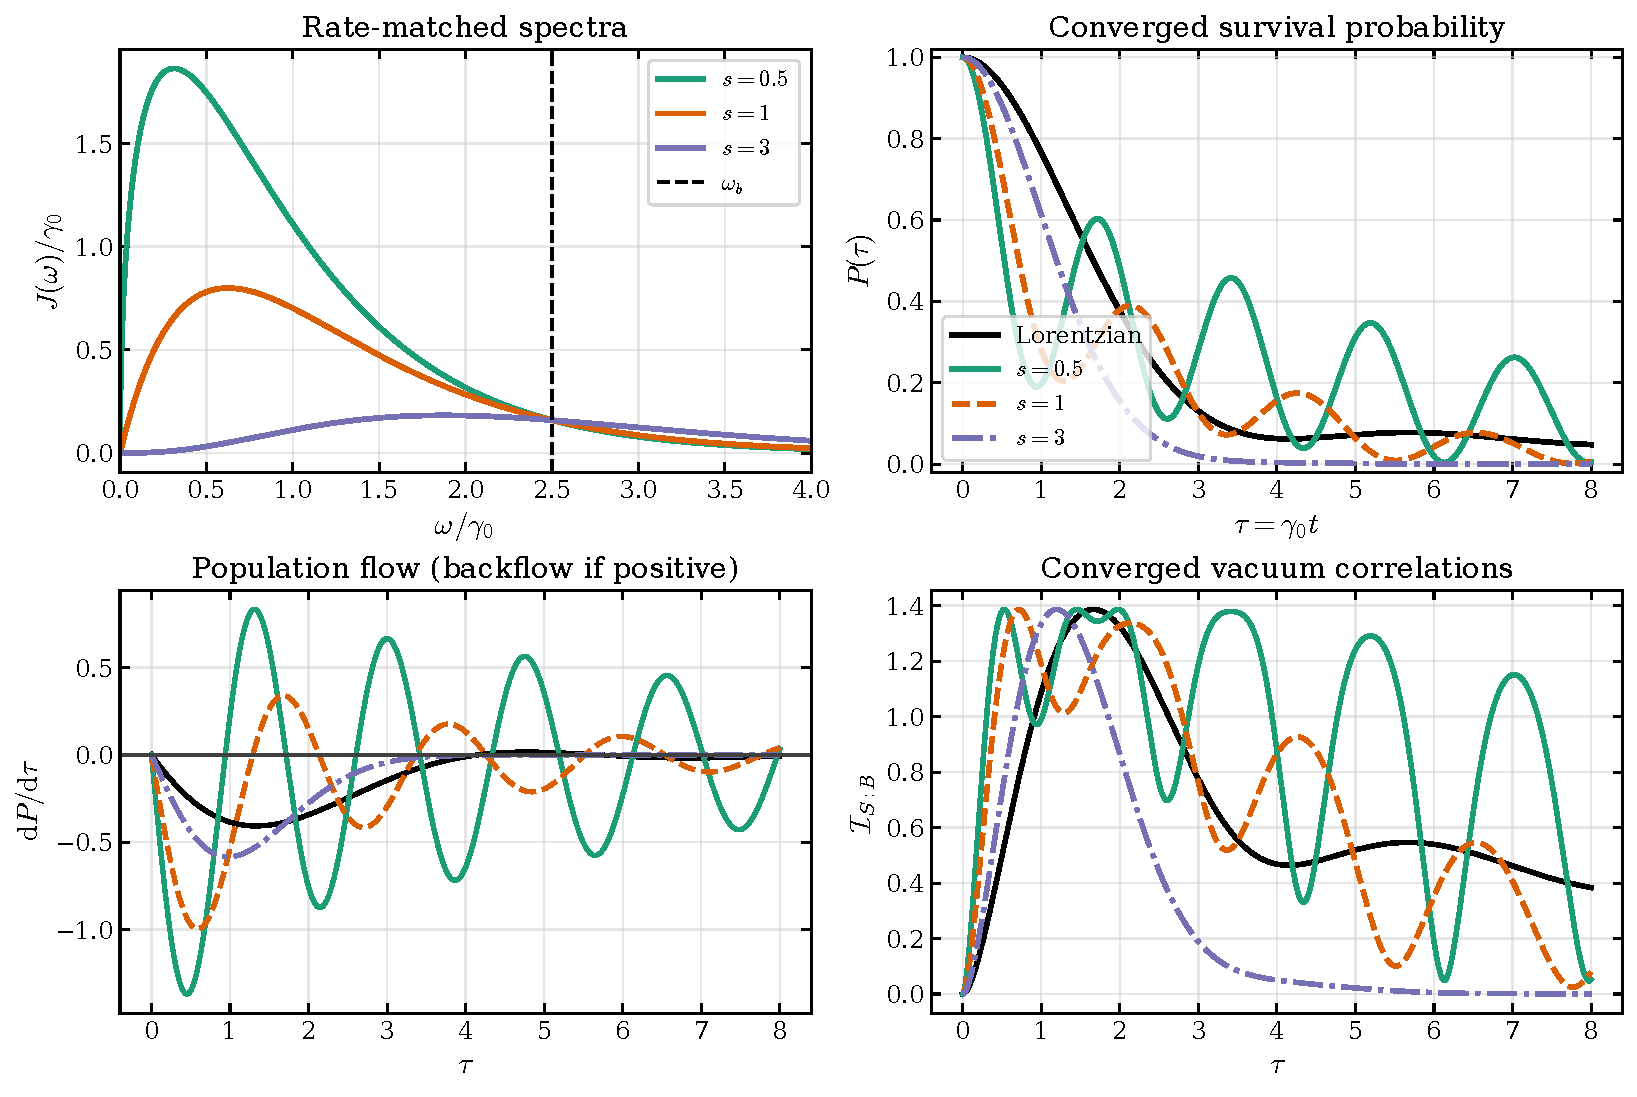
\includegraphics[width=\textwidth]{powerlaw_lorentzian_comparison.pdf}
\caption{Rate-matched spectral densities and their numerically converged
Volterra dynamics. The occurrence and magnitude of revival, final survival, and
correlation dynamics remain spectrally nonuniversal even though the
amplitude-only identities are unchanged.}
\label{fig:powerlawcomparison}
\end{figure*}


\section{Commuting phase damping: a scope check}
\label{sec:phasedamping}

Amplitude damping ties population, bare energy, and trace-distance backflow
together. To delimit the scope of that mechanism, we briefly contrast it
with the known commuting structure of thermal
phase-damping coupling
\begin{equation}
V_\phi=\sigma_z\sum_k(g_kb_k+g_k^*b_k^\dagger),
\label{eq:phasedampinginteraction}
\end{equation}
while retaining the same \(H_S(t)\) and \(H_B\) of the original Hamiltonian~\eqref{M-eq:Hamiltonian}. Since
\([H_S(t),H_S(u)]=[H_S(t),H_B+V_\phi]=0\), the propagator factorizes:
\begin{equation}
U(t)=\exp\left[-\ii\int_0^tH_S(u)\dd u\right]
\exp[-\ii t(H_B+V_\phi)].
\label{eq:phasedampingfactorization}
\end{equation}
For a bath initially in a Gibbs state, the exact reduced coherence is
\begin{align}
\rho_{eg}(t)&=\rho_{eg}(0)\ee^{-\ii\Phi(t)-\Gamma_\beta(t)},
\label{eq:phasecoherence}\\
\Gamma_\beta(t)&=4\int_0^\infty\frac{J(\omega)}{\omega^2}
\coth\left(\frac{\beta\omega}{2}\right)
[1-\cos(\omega t)]\dd\omega.
\label{eq:phaseGamma}
\end{align}
The reduced dissipative map is therefore invariant under every frequency
protocol, up to a system-only phase. Detuning cannot change the coherence
magnitude, dephasing rate, CP divisibility, optimized distinguishability
backflow, or microscopic entropy production. This is an exact no-go result
for detuning-only control of phase damping and is consistent with recent
frequency-modulation analyses~\cite{Khazaei2026}; it is included as a scope
check, not as a second universality claim.

Here \(\mathcal F_\beta(t)\equiv
\Tr[H_S(t)\rho_S(t)]-\beta^{-1}S[\rho_S(t)]\) is the nonequilibrium free
energy of the reduced qubit, and \(\dot W_S\equiv
\Tr[\dot H_S(t)\rho_S(t)]\) is the control-work rate.
Nevertheless, a negative exact dephasing rate can return information. For an
initially coherent qubit,
\begin{align}
\gamma_\phi<0
&\Longleftrightarrow \dot S_S<0\nonumber\\
&\Longleftrightarrow
\dot{\mathcal F}_\beta-\dot W_S=-\beta^{-1}\dot S_S>0,
\qquad \dot Q_S=0.
\label{eq:phasefreeenergy}
\end{align}
Here \(\gamma_\phi=\dot\Gamma_\beta\), and the trace distance between two
states with transverse and longitudinal squared Bloch-vector differences
\(A\) and \(B\) is
\begin{equation}
D_{12}^{(\phi)}=\frac12\sqrt{\ee^{-2\Gamma_\beta}A+B},
\end{equation}
so \(\gamma_\phi<0\) is exactly equivalent to coherence distinguishability
backflow whenever \(A>0\).
Thus phase memory can recharge nonequilibrium free energy through purification
without bare-energy backflow. The two exactly solvable channels isolate two
different mechanisms: bare-energy return for amplitude damping and
information return for phase damping. This distinction is consistent with the multitime
resource hierarchy of Ref.~\cite{ZambonAdesso2025}, while providing a concrete
microscopic realization in which the relevant currents can be evaluated
exactly.


\section{Generated correlations for the reference pure state}

The correlation identities in this section refer specifically to the initial
product state
\begin{equation}
|\Psi(0)\rangle=|e\rangle\otimes|0\rangle_B.
\label{eq:referenceinitialstate}
\end{equation}
Excitation-number conservation then keeps the joint state pure in the
one-excitation sector, with Schmidt weights \(P\) and \(1-P\). Hence the von
Neumann entropies read \(S_S=S_B=h_2(P)\), where
\(h_2(P)=-P\ln P-(1-P)\ln(1-P)\), with
\(S(\rho)=-\Tr(\rho\ln\rho)\). The exact mutual information between the
system and the bosonic reservoir is
\begin{equation}
\I_{S:B}=2h_2(P),
\label{eq:mutualinformation}
\end{equation}
and therefore
\begin{equation}
\dot\I_{S:B}=\frac{2}{\omega}
\ln\left(\frac{1-P}{P}\right)\,\dot Q_S,
\qquad 0<P<1,\quad \omega>0.
\label{eq:energycorrelation}
\end{equation}
The mutual information itself extends continuously to
\(\I_{S:B}=0\) at \(P=0,1\); its derivative at either endpoint must be
evaluated as a trajectory limit rather than by direct substitution in
Eq.~\eqref{eq:energycorrelation}. Positive heat-like return and correlation growth
are not equivalent: the latter changes sign also at \(P=1/2\). A finite
measure of the correlations generated from the initial product state is
\begin{equation}
\mathcal C_{S:B}
=D(\rho_{SB}\Vert\rho_S\otimes\rho_B)
=\I_{S:B}=2h_2(P)\geq0.
\label{eq:correlationentropy}
\end{equation}
It is generated mutual information, not the Clausius entropy production of a
genuinely thermal reservoir. The strong-coupling thermodynamic partition and the
zero-temperature support obstruction are detailed in
Sec.~\ref{app:thermodynamics}.


\section{Experimental implementation details}

A direct experimental test can be implemented with a tunable qubit coupled
to a lossy cavity mode, which realizes the Lorentzian pseudomode in
Eq.~\eqref{M-eq:pseudomode}. One first calibrates \(\gamma_0\) and the cavity
linewidth \(\lambda\), prepares one qubit excitation with the mode near its
vacuum, sets \(\omega(0)=\omega_b\), and applies a chirp over
\(\Delta_f<\omega_b\). As a circuit-QED scale estimate, take
\(\gamma_0/2\pi=50\,\mathrm{MHz}\), \(\ell=5/8\), \(a=5/32\),
\(\Omega_\Delta=5/4\), and \(\Omega_b=100\). These values correspond to
\(\lambda/2\pi=31.25\,\mathrm{MHz}\), a sweep from \(5.000\) to
\(4.9375\,\mathrm{GHz}\) in \(t_f=25.5\,\mathrm{ns}\), and
\(\alpha/2\pi=2.45\,\mathrm{GHz}/\mu\mathrm{s}\). The fractional sweep is
only \(1.25\%\), limiting unwanted variation of the qubit eigenbasis and the
coupling matrix elements; any residual variation of \(g\) can be included as
a calibrated systematic error. At \(20\,\mathrm{mK}\), the thermal
occupation at \(5\,\mathrm{GHz}\) is below \(10^{-5}\), while additional
dephasing is perturbative when \(t_f/T_\phi\ll1\).

Repeated population measurements locate the revival most robustly by fitting
the full time trace to Eq.~\eqref{M-eq:pseudomode}, rather than differentiating
noisy data near a population minimum. Scanning \(\alpha\) and
\(\lambda\) would therefore map the predicted critical lobe, test
the \(a^{1/2}+a^{3/4}\) collapse near its resonant anchor, and resolve the
endpoint cusp by varying the sweep range. Measuring the cavity occupation
and output intensity reconstructs the pseudomode loss
\(2\ell|b|^2\), but not \(E_I\) by itself. The interaction energy requires
the phase-sensitive correlator
\(2\Ree[g\langle\sigma_+b\rangle]\), obtainable from calibrated joint
qubit--cavity tomography or phase-sensitive heterodyne inference. Thus the
population-only boundary test does not require full process tomography,
whereas the microscopic energy partition does.


\section{Other exactly solvable control profiles}
\label{app:exactprofiles}

The waveform universality result can be checked without abandoning exact
solvability. For an arbitrary dimensionless detuning \(\delta(\tau)\), the
single-resonance Lorentzian equation and its gauge transformation are
\begin{align}
c''+(\ell+\ii\delta)c'+\frac{\ell}{2}c&=0,
\label{eq:generalprofileode}\\
c&=\exp\!\left[-\frac{\ell\tau}{2}
-\frac{\ii}{2}\int_0^\tau\delta(u)\dd u\right]y,
\nonumber\\
y''+\bigg[\frac{\ell(2-\ell)}4+\frac{\delta^2}4
&-\frac{\ii}{2}\delta'
\nonumber\\[-2pt]
&-\frac{\ii\ell}{2}\delta\bigg]y=0.
\label{eq:generalprofilegauge}
\end{align}
Equation~\eqref{eq:generalprofilegauge} identifies three further solvable
families, summarized in Table~\ref{tab:exactprofiles}. In each case the
closed form was evaluated independently of direct integration of
Eq.~\eqref{eq:generalprofileode}.

\begin{table*}[t]
\caption{Exactly solvable detuning protocols beyond the linear ramp. Here
\(a=\delta'(0)=d/\theta\) for the two saturating profiles. The last column
gives the first waveform-dependent correction to the linear-ramp boundary.}
\label{tab:exactprofiles}
\begin{ruledtabular}
\begin{tabular}{@{}p{0.19\textwidth}p{0.14\textwidth}
p{0.20\textwidth}p{0.29\textwidth}@{}}
Protocol & Reduced equation & Exact representation & Boundary correction\\
\hline
\(\delta=d\tanh(\tau/\theta)\)
& complex Rosen--Morse & Gauss \({}_2F_1\)
& \(\ell_c^{\tanh}-\ell_c^{\rm lin}
=(\pi^2-3)a^2/(6d^2)+o(a^2)\)\\
\(\delta=d(1-\ee^{-\tau/\theta})\)
& Morse & Whittaker \(M_{\kappa,\mu},W_{\kappa,\mu}\)
& \(\ell_c^{\exp}-\ell_c^{\rm lin}
=K_2a^{5/4}/(2d)+o(a^{5/4})\)\\
Piecewise affine double passage
& Weber on each segment & product of Weber transfer matrices
& not in the monotone-profile theorem\\
\end{tabular}
\end{ruledtabular}
\end{table*}

For the exponential profile,
\begin{equation}
K_2=\frac{2^{7/4}(2\pi^2-3)}{12\sqrt\pi}
=2.6471663693\ldots .
\label{eq:Ktwoappendix}
\end{equation}
Both saturating protocols therefore retain the entire
\(a^{1/2}+a^{3/4}\) law; their shape first becomes visible only at the higher
orders displayed in Table~\ref{tab:exactprofiles}. At
\((\ell,d,\theta)=(0.625,0.625,4)\), the maximum discrepancies between the
special-function and direct-ODE results are
\begin{align}
\max|c_{{}_2F_1}-c_{\rm ODE}|&=5.82\times10^{-12},
\nonumber\\
\max|q_{{}_2F_1}-q_{\rm ODE}|&=3.86\times10^{-11},
\nonumber\\
\max|c_W-c_{\rm ODE}|&=6.57\times10^{-12},
\nonumber\\
\max|q_W-q_{\rm ODE}|&=5.11\times10^{-11}.
\label{eq:profilevalidation}
\end{align}

For a segment with nonzero constant slope \(v\), let \(F_v\) denote the
fundamental matrix built from the two Weber solutions. Its exact transfer
matrix is
\begin{equation}
T_v(\delta_a\!\to\!\delta_b)
=F_v(\delta_b/v)F_v(\delta_a/v)^{-1}.
\label{eq:webertransfer}
\end{equation}
Products of Eq.~\eqref{eq:webertransfer} solve triangular, staircase, and
repeated-passage controls. A representative triangular double passage gives
\(\mathcal N_P=0.0163081\), while agreeing with direct
integration within \(6.5\times10^{-12}\). Because a second passage can create
a later and distinct revival, this example also shows why monotonicity and
positive saturation are substantive hypotheses of the uniform slow-sweep
argument, not
merely technical conveniences.

\section{Finite sums of displaced Lorentzian resonances}
\label{app:multilorentzian}

The single-resonance construction has an exact finite-dimensional extension. For
a positive sum of Lorentzian densities,
\begin{equation}
J_N(\omega)=\sum_{j=1}^N
\frac{\gamma_j\lambda_j^2}
{2\pi[(\omega-\omega_j)^2+\lambda_j^2]},
\label{eq:multilorentzianJ}
\end{equation}
the vacuum amplitude is represented by \(N\) damped pseudomodes
\cite{Garraway1997,Pleasance2020}:
\begin{align}
c'&=-\ii\sum_{j=1}^Ng_jb_j,
\nonumber\\
b_j'&=-[\ell_j+\ii\delta_j(\tau)]b_j-\ii g_jc,
\label{eq:multipseudomode}\\
\frac{\dd}{\dd\tau}\left(|c|^2+\sum_j|b_j|^2\right)
&=-2\sum_j\ell_j|b_j|^2\leq0.
\label{eq:multipseudomodenorm}
\end{align}
Thus every channel, energetic, and correlation identity that depends only on
\(c\) remains exact for the multi-Lorentzian reservoir.

We tested the critical law on the co-centered two-Lorentzian family
\begin{equation}
\frac{J_2(\omega)}{\gamma_0}
=\sum_{j=1}^2\frac{w_j\ell_j^2}
{2\pi[x^2+\ell_j^2]},\qquad
x=\frac{\omega-\omega_b}{\gamma_0},
\label{eq:bilorentzianfamily}
\end{equation}
with \((w_1,w_2)=(0.65,0.35)\),
\((\ell_1,\ell_2)=r(1,3)\), and
\(g_j^2=w_j\ell_j/2\). At zero detuning the secular function is
\begin{equation}
F(\sigma;r)=\sigma+\sum_{j=1}^2
\frac{g_j^2}{\sigma+\ell_j}.
\label{eq:multisecular}
\end{equation}
The double-root conditions \(F=\partial_\sigma F=0\) give
\begin{equation}
\sigma_*=-0.938929647080,\qquad r_*=1.702728289304,
\label{eq:biep}
\end{equation}
while the remaining eigenvalue is \(-4.93305386306\), well separated from
the exceptional pair. The isolated pair therefore supplies the same local
two-dimensional exceptional-point normal form as the single-resonance case; the
spectator mode renormalizes its coefficients.

High-precision continuation of the exact double-tangency conditions for a
common chirp \(\delta_j=a\tau\), over
\(10^{-6}\leq a\leq10^{-2}\), gives
\begin{align}
r_c(a)=r_*&-4.3699457a^{1/2}
+1.2071935a^{3/4}
\nonumber\\
&+0.5942697a+o(a).
\label{eq:bilorentzianfit}
\end{align}
The fit uses \(a\leq10^{-3}\) and has maximum relative error
\(1.6\times10^{-4}\) on that interval. The local logarithmic slope of
\(r_*-r_c\) approaches \(1/2\) from below. The leading exponent is therefore
unchanged, whereas all displayed coefficients are spectral and the
\(a^{3/4}\) coefficient in Eq.~\eqref{eq:bilorentzianfit} is a numerical
result, not a claimed multi-Lorentzian universality theorem.

\begin{figure*}[t]
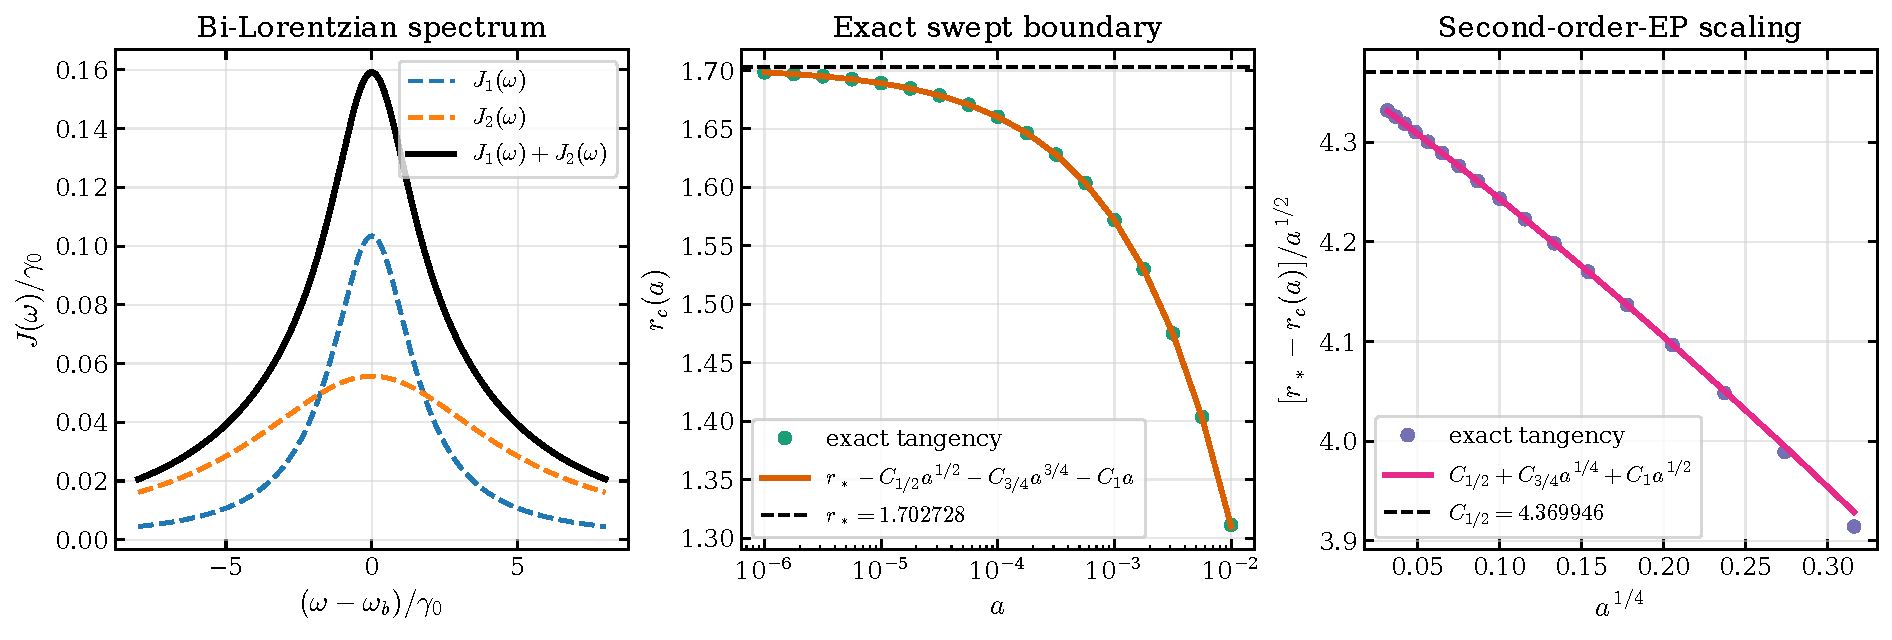
\includegraphics[width=\textwidth]{bilorentzian_boundary.pdf}
\caption{Two-pseudomode test. Left: the positive bi-Lorentzian density
and its two components. Center: numerically continued exact tangency
conditions and fractional-power fit. Right: normalization by \(a^{1/2}\)
exposes convergence to the leading
exceptional-point coefficient.}
\label{fig:bilorentzian}
\end{figure*}

Equations~\eqref{eq:multilorentzianJ}--\eqref{eq:multipseudomode} do not imply
that every spectral density is globally and exactly a finite positive
Lorentzian sum. They give a controlled route for spectra whose bath
correlation function is exactly represented, or approximated on a prescribed
time window, by a finite exponential expansion. The approximation error and
the structural stability of the critical boundary must then be checked
separately. Figure~\ref{fig:bilorentzian} establishes the first nontrivial
finite-sum case and supports, without overstating, extension to rational
pseudomode approximations of more complicated reservoirs.

\section{Strong-coupling entropy partition and vacuum limit}
\label{app:thermodynamics}

For a factorized initial state with a bath genuinely prepared at inverse
temperature \(\beta\), unitary global dynamics gives the exact identity
\begin{equation}
\Sigma_{\rm mic}(t):=\Delta S_S+\beta\Delta E_B
=\I_{S:B}+D(\rho_B(t)\Vert\rho_B^\beta)\geq0.
\label{eq:microscopicentropy}
\end{equation}
This correlation--displacement decomposition is the microscopic form of
entropy production at arbitrary coupling
\cite{Esposito2010,Ptaszynski2019}.
At finite coupling this differs from the reduced Clausius expression because
\(Q_S=-\Delta E_B-E_I\):
\begin{equation}
\Sigma_{\rm red}:=\Delta S_S-\beta Q_S
=\Sigma_{\rm mic}+\beta E_I.
\label{eq:entropypartition}
\end{equation}
Only \(\Sigma_{\rm mic}\) possesses the universally nonnegative decomposition
in Eq.~\eqref{eq:microscopicentropy}.

For a diagonal qubit, define
\begin{equation}
\mathcal F_\beta(P,t)=\omega(t)P-\beta^{-1}h_2(P),
\qquad
p_\beta(t)=\frac1{1+\ee^{\beta\omega(t)}}.
\end{equation}
The change not supplied as explicit control work is
\begin{equation}
\dot{\mathcal F}_\beta-\dot W_S
=\beta^{-1}\dot P
\ln\frac{P(1-p_\beta)}{p_\beta(1-P)}.
\label{eq:freeenergycriterion}
\end{equation}
During a revival interval \(\dot P>0\), the bare qubit is recharged in
nonequilibrium free energy if and only if \(P>p_\beta\). This is not yet a
net-work theorem: sudden removal of the interaction costs
\begin{equation}
W_{\rm off}=-E_I.
\end{equation}
For the positive-carrier representative trajectory, the end of the revival
has \(W_{\rm off}/\gamma_0=0.0219236\), while
\(\mathcal Q_{S,+}/\gamma_0=0.3066815\). Their ordering depends on
the independent carrier \(\Omega_b\) and is not by itself a work statement:
the full extraction, switching, and reset cycle is still unspecified. Thus
the integrated positive heat-like current cannot be called extractable work from this
comparison alone.

The exact amplitude solution in the main text assumes the pure vacuum. Once
an excitation has entered the bath,
\begin{equation}
D(\rho_B(t)\Vert |0\rangle\langle0|)=+\infty.
\end{equation}
Accordingly, the conventional dimensionless thermal entropy production is
singular as \(\beta\to\infty\). The finite zero-temperature rate remaining
after division by \(\beta\) is \(-\dot Q_S\) for the reduced partition and
\(\dot E_B=-\dot Q_S-\dot E_I\) for the microscopic partition. The finite
quantity in Eq.~\eqref{eq:correlationentropy} is instead generated mutual
information, not a Clausius entropy production.

\section{Numerical methods and convergence}
\label{app:numerics}

The Lorentzian boundary was computed in three independent ways: direct
integration of Eq.~\eqref{M-eq:exactODE}, integration of
Eq.~\eqref{M-eq:Riccati} with variational equations for the double-root
conditions, and arbitrary-precision evaluation of Eq.~\eqref{eq:qWeber}.
The slow-sweep representation removes the dominant exponential before
integration. The endpoint cusp was obtained from
\(g=\partial_\ell g=0\), with derivatives evaluated from the exact
variational system rather than finite differencing a phase grid.
The scripts \texttt{finite\_sweep\_phase\_boundary.py} and
\texttt{sweep\_range\_dependence.py} record seeds, tolerances, and the
mechanism-switch, endpoint-birth, cusp-tip, and range-crossover data reported
in the main text, in Eq.~\eqref{eq:rangecrossover}, and in
Table~\ref{tab:rangedependence}. The independent regression script
\texttt{verify\_key\_results.py} checks all three characteristic points and
the sign-resolved energy balance reported in the main text.
The separate script \texttt{verify\_table\_ii.py} recomputes the Lorentzian
row of Table~\ref{tab:powerlaw} on a 20001-point grid and verifies
\(\mathcal N_P\) and \(\mathcal Q_{S,+}\) both by direct quadrature and by the
independent integration-by-parts formula in Eq.~\eqref{eq:Ebackparts}.

For the power-law reservoirs, Eq.~\eqref{eq:Volterra} was advanced with a
second-order trapezoidal product-integration rule. At each time step the
implicit endpoint contribution was iterated to convergence. The analytical
bath transform in Eq.~\eqref{eq:powerlawkernel} was used directly, avoiding a
frequency discretization. The trajectories in Table~\ref{tab:powerlaw} use
5000 time intervals. Halving the step changes the entire population curve
by less than \(5.97\times10^{-6}\) and \(\mathcal N_P\) by less than
\(3.87\times10^{-6}\) for \(s=0.5,1,3\). These coarse--fine differences,
the individual \(\alpha_B\) values, and the common final time are reported in
Table~\ref{tab:powerlaw}.

All plotted Lorentzian phase boundaries are sign boundaries of the exact
Lorentzian-reservoir rate. No finite positive cutoff was used to define the existence of a
revival. Phase-diagram contours of integrated revival, where present, are
observables inside the already determined domain and do not define its edge.

\section{Exact reservoir amplitudes and microscopic bath reconstruction}
\label{app:reservoir_amplitudes}

This section reconstructs a finite microscopic star reservoir
from the continuum Lorentzian model and derives every reservoir-mode
amplitude. We keep two frequencies distinct throughout. The quantity
\(\omega_S(t)\) is the instantaneous two-level-system (TLS) gap, whereas
\(\omega_b\) is the center of the reservoir spectral density. In general,
\begin{equation}
\omega_S(t)\ne\omega_b,
\qquad \delta(t)=\omega_b-\omega_S(t).
\label{eq:s_detuning}
\end{equation}
Only the resonant linear protocol studied in the main text imposes the
initial condition \(\omega_S(0)=\omega_b\), after which
\(\omega_S(t)=\omega_b-\alpha t\) and \(\delta(t)=\alpha t\). On the
finite protocol of the main text,
\(0\leq t\leq\Delta_f/\alpha\), so
\(\omega_S(t)\geq\omega_f=\omega_b-\Delta_f>0\).

\subsection{General control waveform}

Consider the rotating-wave Hamiltonian
\begin{equation}
\begin{aligned}
H(t)={}&\omega_S(t)\sigma_+\sigma_-+\sum_k\omega_k b_k^\dagger b_k\\
&+\sum_k\left(g_k\sigma_+b_k+g_k^*\sigma_-b_k^\dagger\right).
\end{aligned}
\label{eq:s_H}
\end{equation}
Excitation-number conservation confines an initial state \(|e,0\rangle\) to
the one-excitation sector,
\begin{equation}
|\Psi(t)\rangle=C_e(t)|e,0\rangle
+\sum_k C_k(t)|g,1_k\rangle.
\label{eq:s_state}
\end{equation}
Define
\begin{equation}
\begin{aligned}
\Phi(t)&=\int_0^t\omega_S(v)\dd v,\\
C_e(t)&=c(t)\ee^{-\ii\Phi(t)},\qquad
C_k(t)=\beta_k(t)\ee^{-\ii\omega_kt}.
\end{aligned}
\label{eq:s_phases}
\end{equation}
Direct substitution into the Schr\"odinger equation gives
\begin{align}
\dot c(t)&=-\ii\sum_k g_k\beta_k(t)
 \ee^{-\ii[\omega_kt-\Phi(t)]},
\label{eq:s_cdot}\\
\dot\beta_k(t)&=-\ii g_k^*c(t)
 \ee^{\ii[\omega_kt-\Phi(t)]}.
\label{eq:s_betadot}
\end{align}
Therefore, once the exact atomic amplitude is known, every microscopic bath
coefficient follows from the single quadrature
\begin{equation}
\begin{aligned}
\beta_k(t)&=-\ii g_k^*\int_0^t c(u)
\exp\!\left\{\ii\left[\omega_ku-\Phi(u)\right]\right\}\dd u,\\
C_k(t)&=\beta_k(t)\ee^{-\ii\omega_kt}.
\end{aligned}
\label{eq:s_beta_general}
\end{equation}
Equation~\eqref{eq:s_beta_general} is exact for an arbitrary differentiable
control waveform and makes no assumption relating \(\omega_b\) to the TLS
frequency. It also fixes the phase convention unambiguously: changing the
definition of the interaction-picture coefficients changes the exponential
signs in both Eqs.~\eqref{eq:s_cdot} and \eqref{eq:s_beta_general}, but leaves
the Schr\"odinger-picture state invariant.

The coefficient equations immediately imply the microscopic normalization
identity
\begin{equation}
|c(t)|^2+\sum_k|\beta_k(t)|^2=1.
\label{eq:s_norm}
\end{equation}
Thus the continuum survival probability alone determines the total emitted
population, while Eq.~\eqref{eq:s_beta_general} resolves how that population
is distributed among reservoir modes.

\subsection{Linear chirp and the Weber solution}

For the protocol of the main text,
\begin{equation}
\omega_S(t)=\omega_b-\alpha t,\qquad
\Phi(t)=\omega_bt-\frac{\alpha t^2}{2}.
\label{eq:s_linear}
\end{equation}
Writing \(\Omega_k=\omega_k-\omega_b\), Eq.~\eqref{eq:s_beta_general}
becomes
\begin{equation}
\beta_k(t)=-\ii g_k^*\int_0^t c(u)
\ee^{\ii\Omega_ku+\ii\alpha u^2/2}\dd u.
\label{eq:s_beta_linear_dimensional}
\end{equation}
Introduce
\begin{equation}
\begin{gathered}
\tau=\gamma_0t,\qquad
x_k=\frac{\omega_k-\omega_b}{\gamma_0},\qquad
\widetilde g_k=\frac{g_k}{\gamma_0},\\
\ell=\frac{\lambda}{\gamma_0},\qquad
a=\frac{\alpha}{\gamma_0^2}.
\end{gathered}
\label{eq:s_dimensionless}
\end{equation}
Then
\begin{equation}
\beta_k(\tau)=-\ii\widetilde g_k^*\int_0^\tau c(v)
\ee^{\ii x_kv+\ii av^2/2}\dd v.
\label{eq:s_beta_dimensionless}
\end{equation}
The exact atomic amplitude is
\begin{align}
c(v)&=\ee^{-\ell v/2-\ii av^2/4}
\left[A D_\nu(z(v))+B D_\nu(-z(v))\right],
\label{eq:s_weber}\\
\nu&=\ii\frac{\ell}{2a},\qquad
z(v)=\ee^{-\ii\pi/4}\sqrt a
\left(v-\frac{\ii\ell}{a}\right),
\label{eq:s_weber_parameters}
\end{align}
where \(A\) and \(B\) are fixed by \(c(0)=1\) and \(c'(0)=0\).
With
\(z_0=-\ee^{-\ii\pi/4}\ii\ell/\sqrt a\) and
\(\eta=\ee^{-\ii\pi/4}\sqrt a\), these coefficients are the unique
solution of
\begin{equation}
\begin{pmatrix}
D_\nu(z_0)&D_\nu(-z_0)\\
\eta D_\nu'(z_0)&-\eta D_\nu'(-z_0)
\end{pmatrix}
\begin{pmatrix}A\\B\end{pmatrix}
=\begin{pmatrix}1\\\ell/2\end{pmatrix}.
\label{eq:ABsystem}
\end{equation}
Using \(D_\nu'(z)=zD_\nu(z)/2-D_{\nu+1}(z)\), the logarithmic derivative
is evaluated without numerical differentiation as
\begin{equation}
q=-\frac\ell2-\frac{\ii a\tau}{2}
+\eta\frac{A D_\nu'(z)-B D_\nu'(-z)}
{A D_\nu(z)+B D_\nu(-z)}.
\label{eq:qWeber}
\end{equation}
For very small \(a\), direct special-function evaluation becomes
ill-conditioned because \(\nu=\ii\ell/(2a)\) has large imaginary order. We
therefore use Eq.~\eqref{M-eq:exactODE}, its exponentially desingularized
form, and Eq.~\eqref{M-eq:Riccati} as independent numerical
representations. At \(a=10^{-2}\), their values of \(q\) at the critical
tangency agree within \(3.2\times10^{-12}\).

Substitution gives the exact mode-resolved representation
\begin{align}
\beta_k(\tau)&=-\ii\widetilde g_k^*
\left[A I_{k,+}(\tau)+B I_{k,-}(\tau)\right],
\label{eq:s_beta_weber}\\
I_{k,\pm}(\tau)&=\int_0^\tau
\ee^{-\ell v/2+\ii x_kv+\ii av^2/4}
D_\nu(\pm z(v))\dd v.
\label{eq:s_Ik}
\end{align}
The sign of the damping factor in Eq.~\eqref{eq:s_Ik} follows directly from
Eq.~\eqref{eq:s_weber}; it is therefore not an independent convention.

For a closed special-function representation, define the entire functions
\begin{equation}
F_\pm(v)=\ee^{-\ell v/2+\ii av^2/4}D_\nu(\pm z(v))
=\sum_{m=0}^\infty d_m^{(\pm)}v^m,
\label{eq:s_Fseries}
\end{equation}
with coefficients
\begin{equation}
d_m^{(\pm)}=\frac{1}{m!}
\left.\frac{\dd^m}{\dd v^m}F_\pm(v)\right|_{v=0}.
\label{eq:s_dm}
\end{equation}
Because \(D_\nu(z)\) is entire in \(z\) for fixed \(\nu\), this series
converges uniformly on every finite time interval. Termwise integration is
therefore legitimate and yields, for \(x_k\ne0\),
\begin{equation}
I_{k,\pm}(\tau)=\sum_{m=0}^\infty d_m^{(\pm)}
\frac{\gamma(m+1,-\ii x_k\tau)}{(-\ii x_k)^{m+1}},
\label{eq:s_incomplete_gamma}
\end{equation}
where \(\gamma(s,z)=\int_0^z y^{s-1}\ee^{-y}\dd y\) is the lower
incomplete gamma function on a consistent branch. The resonant-mode limit
is regular and is best evaluated as
\begin{equation}
I_{0,\pm}(\tau)=\sum_{m=0}^\infty
d_m^{(\pm)}\frac{\tau^{m+1}}{m+1}.
\label{eq:s_incomplete_gamma_zero}
\end{equation}
Equations~\eqref{eq:s_beta_weber}--\eqref{eq:s_incomplete_gamma_zero} are an
exact incomplete-gamma realization of the hypergeometric/Pochhammer
expansion derived in the original notes, but avoid storing a triple-index
coefficient array. Near \(x_k=0\), Eq.~\eqref{eq:s_Ik} or
Eq.~\eqref{eq:s_incomplete_gamma_zero} should be used to avoid cancellation.

\section{From the Lorentzian continuum to a finite star bath}
\label{app:discretization}

The continuum density is
\begin{equation}
J_L(\omega)=\frac{\gamma_0\lambda^2}
{2\pi[(\omega-\omega_b)^2+\lambda^2]}
=\frac{\gamma_0\lambda}{2}L_\lambda(\omega-\omega_b),
\label{eq:s_J}
\end{equation}
where
\begin{equation}
L_\eta(x)=\frac{1}{\pi}\frac{\eta}{x^2+\eta^2},
\qquad \int_{-\infty}^{\infty}L_\eta(x)\dd x=1.
\label{eq:s_L}
\end{equation}
A finite star Hamiltonian is specified by representative frequencies
\(\omega_k\) and couplings \(g_k\). Let the frequency axis be partitioned
into cells \(\mathcal C_k=[\omega_{k,-},\omega_{k,+}]\), with
\(\omega_k\in\mathcal C_k\). The most direct continuum quadrature is
\begin{equation}
|g_k|^2=\int_{\mathcal C_k}J_L(\omega)\dd\omega,
\qquad g_k=\ee^{\ii\phi_k}\sqrt{|g_k|^2}.
\label{eq:s_cell_general}
\end{equation}
For the Lorentzian, the cell integral is elementary:
\begin{equation}
|g_k|^2=\frac{\gamma_0\lambda}{2\pi}
\left[
\arctan\!\frac{\omega_{k,+}-\omega_b}{\lambda}
-\arctan\!\frac{\omega_{k,-}-\omega_b}{\lambda}
\right].
\label{eq:s_cell_exact}
\end{equation}
This exact cell mass is preferable to the midpoint approximation
\begin{equation}
|g_k|^2\simeq J_L(\omega_k)\Delta\omega_k
\label{eq:s_midpoint}
\end{equation}
when the grid is not extremely fine. The phases \(\phi_k\) do not enter
\(J_L\). For a star bath with no independent phase constraints they can be
absorbed into the definitions of the mode operators, so one may set
\(\phi_k=0\).

In the rotating detuning coordinate
\(x=(\omega-\omega_b)/\gamma_0\),
\begin{equation}
j_L(x):=\frac{J_L(\omega_b+\gamma_0x)}{\gamma_0}
=\frac{\ell^2}{2\pi(x^2+\ell^2)}.
\label{eq:s_j_dimensionless}
\end{equation}
For a uniform grid of spacing \(\Delta x\), Eq.~\eqref{eq:s_cell_exact}
becomes
\begin{equation}
|\widetilde g_k|^2=\frac{\ell}{2\pi}
\left[
\arctan\!\frac{x_k+\Delta x/2}{\ell}
-\arctan\!\frac{x_k-\Delta x/2}{\ell}
\right].
\label{eq:s_cell_dimensionless}
\end{equation}
The finite-star equations are simply Eqs.~\eqref{eq:s_cdot} and
\eqref{eq:s_betadot} with the frequencies and couplings from
Eq.~\eqref{eq:s_cell_exact}. Equivalently, for the linear protocol,
\begin{align}
c'(\tau)&=-\ii\sum_k\widetilde g_k\beta_k(\tau)
\ee^{-\ii(x_k\tau+a\tau^2/2)},
\nonumber\\
\beta_k'(\tau)&=-\ii\widetilde g_k^*c(\tau)
\ee^{\ii(x_k\tau+a\tau^2/2)}.
\label{eq:s_star_odes}
\end{align}
These equations conserve Eq.~\eqref{eq:s_norm} exactly; any norm drift is a
numerical integration error rather than a continuum-discretization error.

\subsection{Window, resolution, and recurrence controls}

For a finite window \([\omega_{\min},\omega_{\max}]\), the retained fraction
of the full-line Lorentzian weight is
\begin{equation}
M=\frac{1}{\pi}\left[
\arctan\!\frac{\omega_{\max}-\omega_b}{\lambda}
-\arctan\!\frac{\omega_{\min}-\omega_b}{\lambda}
\right].
\label{eq:s_window_mass}
\end{equation}
The omitted spectral fraction is \(1-M\). For the symmetric dimensionless
window \([-X,X]\),
\begin{equation}
M_X=\frac{2}{\pi}\arctan\frac{X}{\ell}.
\label{eq:s_symmetric_mass}
\end{equation}
A uniform frequency grid also produces a recurrence at approximately
\begin{equation}
T_{\mathrm{rec}}\simeq\frac{2\pi}{\Delta\omega},
\qquad
\tau_{\mathrm{rec}}\simeq\frac{2\pi}{\Delta x}.
\label{eq:s_recurrence}
\end{equation}
Consequently, a controlled calculation requires both small tail weight and
\(\tau_f<\tau_{\mathrm{rec}}\). Stability should be checked by increasing
\(X\) and decreasing \(\Delta x\) independently.

\subsection{Effective full-line Lorentzian reservoir versus positive physical frequencies}
\label{sec:s_positive}

The exponential kernel and exact pseudomode of the main text follow from the
standard analytic extension of Eq.~\eqref{eq:s_J} to
\(\omega\in\mathbb R\). A microscopic bosonic bath with a Hamiltonian
bounded from below instead has \(\omega_k>0\). The positive-frequency
Lorentzian weight is exactly
\begin{equation}
\int_0^\infty J_L(\omega)\dd\omega
=\frac{\gamma_0\lambda}{2}
\left[\frac{1}{2}+\frac{1}{\pi}
\arctan\!\left(\frac{\omega_b}{\lambda}\right)\right].
\label{eq:s_positive_mass}
\end{equation}
Therefore the positive-frequency bath approaches the effective full-line
Lorentzian reservoir
when \(\omega_b/\lambda\gg1\). At finite \(\omega_b/\lambda\), truncating
the grid at \(\omega=0\), or \(x=-\omega_b/\gamma_0\), defines a physically
distinct kernel and should not be advertised as exactly identical to the
single-resonance Lorentzian model. Conversely, a full-line detuning grid
exactly reconstructs the effective full-line Lorentzian reservoir; it
corresponds to a strictly positive laboratory
spectrum whenever the chosen window satisfies
\(\omega_b>\gamma_0X\). Negative detunings \(x_k<0\) by themselves do not
mean negative laboratory frequencies.

\section{Broadening is a visualization problem, not a dynamical quadrature}
\label{sec:s_broadening}

It is often useful to display the discrete measure using narrow Lorentzians,
\begin{equation}
J_{\sigma,N}(\omega)=\sum_k|g_k|^2
L_\sigma(\omega-\omega_k).
\label{eq:s_broadened}
\end{equation}
This operation must be distinguished from choosing the Hamiltonian
couplings. Lorentzians satisfy
\begin{equation}
(L_a*L_b)(x)=L_{a+b}(x).
\label{eq:s_convolution}
\end{equation}
Thus broadening weights sampled directly from the target \(L_\lambda\) by a
kernel \(L_\sigma\) produces a line of width \(\lambda+\sigma\), not
\(\lambda\). To reconstruct the target line after broadening, one instead
samples the deconvolved envelope
\begin{equation}
\mu(\omega)=\frac{\gamma_0\lambda}{2}
L_{\lambda-\sigma}(\omega-\omega_b),
\qquad 0<\sigma<\lambda,
\label{eq:s_deconvolved}
\end{equation}
and uses
\begin{equation}
|g_k^{(\mathrm{plot})}|^2\simeq\mu(\omega_k)\Delta\omega.
\label{eq:s_plot_weights}
\end{equation}
One then has
\(\mu*L_\sigma=(\gamma_0\lambda/2)L_\lambda\) in the continuum limit.
A smooth display requires \(\Delta\omega\lesssim\sigma\ll\lambda\).
The superscript in Eq.~\eqref{eq:s_plot_weights} is deliberate: for the
actual star dynamics one should use the direct cell weights
Eq.~\eqref{eq:s_cell_exact}; the deconvolved weights are required only when
finite-width kernels are used to visualize the delta peaks.

\section{Numerical validation and microscopic energy resolution}
\label{sec:s_validation}

Figure~\ref{fig:s_reconstruction} tests the construction for
\((\ell,a)=(5/8,5/32)\) up to the observation time
\(\tau_{\max}=8\). The exact-cell star baths use
\((N,X)=(200,8),(400,14),(800,20)\). The maximum population errors relative
to the exact pseudomode are, respectively,
\(2.66\times10^{-4}\), \(1.54\times10^{-4}\), and
\(7.92\times10^{-5}\); the largest normalization error is below
\(1.0\times10^{-11}\). These numbers are not fitting parameters: the
couplings are fixed entirely by Eq.~\eqref{eq:s_cell_dimensionless}.

\begin{figure*}[t]
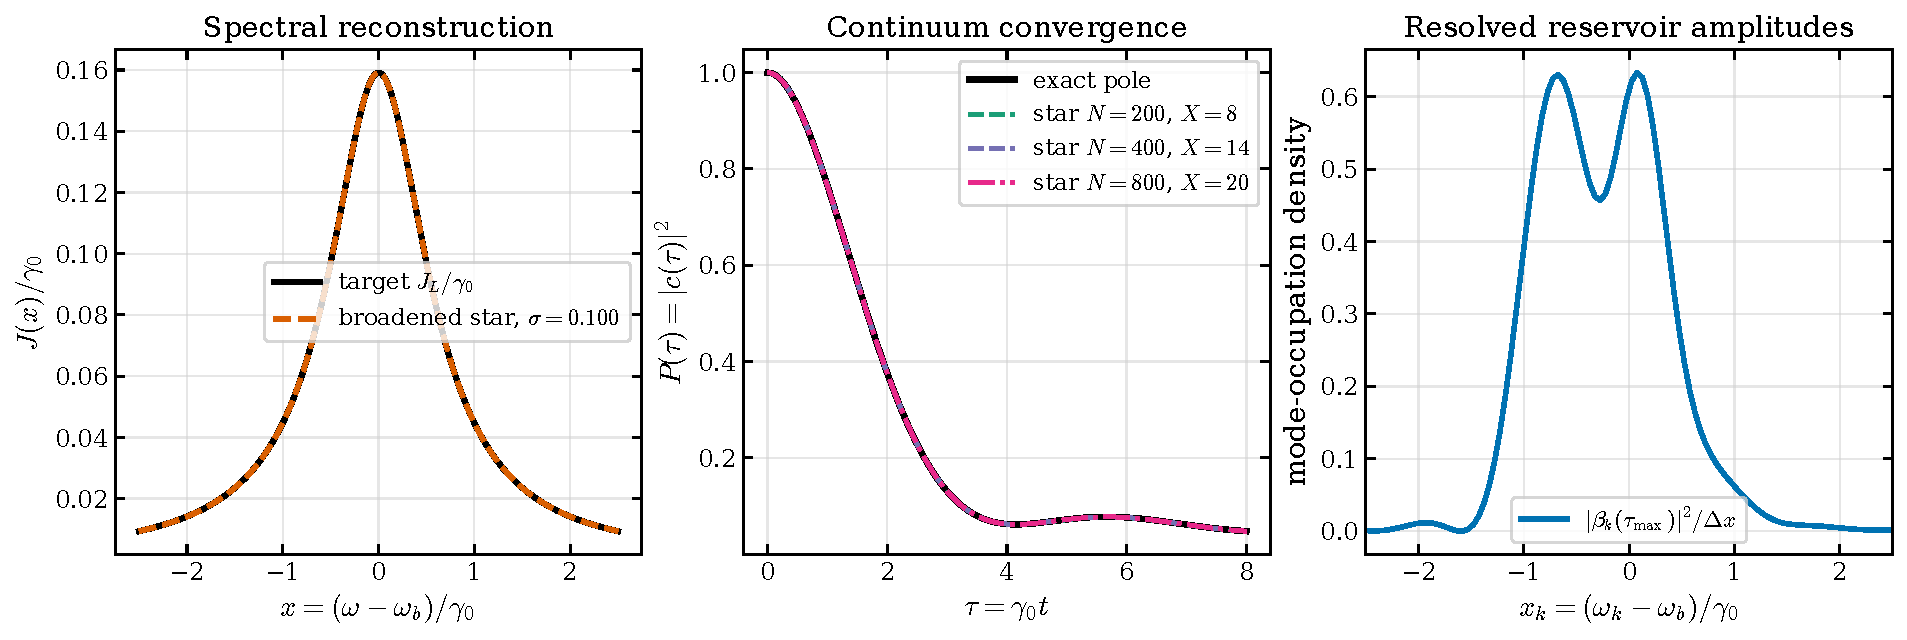
\includegraphics[width=\textwidth]{discrete_bath_reconstruction.pdf}
\caption{Finite-star reconstruction of the effective full-line Lorentzian
reservoir. Left:
the target spectral density (solid black) and its broadened discrete
reconstruction using the deconvolved envelope of
Eq.~\eqref{eq:s_deconvolved} (dashed orange). Center: convergence of the TLS
population from exact-cell star baths to the exact pseudomode result. Right:
the mode-resolved occupation density at \(\tau_{\max}=8\) for the finest star.
The two peaks demonstrate that the final reservoir state is not specified by
the spectral density alone; it also resolves the frequency history of the
controlled emission.}
\label{fig:s_reconstruction}
\end{figure*}

The recovered amplitudes give microscopic access to the reservoir and
interaction energies,
\begin{align}
E_B(t)&=\sum_k\omega_k|\beta_k(t)|^2,
\label{eq:s_EB}\\
E_I(t)&=2\Ree\left[c^*(t)\sum_k g_k\beta_k(t)
\ee^{-\ii[\omega_kt-\Phi(t)]}\right].
\label{eq:s_EI_explicit}
\end{align}
Using Eq.~\eqref{eq:s_cdot}, the interaction energy reduces to an atomic
identity,
\begin{equation}
\begin{aligned}
E_I(t)&=-2\Imm[c^*(t)\dot c(t)]\\
&=-2P(t)\Imm\!\left[\frac{\dot c(t)}{c(t)}\right]
=2P(t)s(t),
\end{aligned}
\label{eq:s_EI_atomic}
\end{equation}
where \(P=|c|^2\) and
\(s=-\Imm(\dot c/c)\) is the exact Lamb-shift function used in the main
text. This equation supplies a mode-resolved numerical check of the purely
atomic thermodynamic relation.

Finally,
\begin{equation}
E_S(t)=\omega_S(t)P(t),\qquad
\dot W(t)=\dot\omega_S(t)P(t),
\label{eq:s_ES_work}
\end{equation}
and unitary evolution under Eq.~\eqref{eq:s_H} gives the exact first-law
balance
\begin{equation}
\dot E_S+\dot E_B+\dot E_I=\dot W,
\qquad
\dot E_B+\dot E_I=-\omega_S(t)\dot P(t).
\label{eq:s_first_law}
\end{equation}
Hence the finite-star reconstruction does more than reproduce \(P(t)\): it
separates the energy stored in the reservoir modes from the generally
non-negligible interaction energy, while their sum exactly matches the
heat-like atomic power. This is precisely the separation lost if one keeps
only a time-local Markovian decay rate.

\subsection{Reproducibility}

The script \texttt{discrete\_bath\_reconstruction.py} generates
Fig.~\ref{fig:s_reconstruction} and the accompanying convergence and
mode-resolved data tables. It integrates both the two-dimensional exact
pseudomode system and the finite star equations
Eq.~\eqref{eq:s_star_odes} with identical physical parameters.


\begin{thebibliography}{99}

\bibitem{Breuer2009}
H.-P. Breuer, E.-M. Laine, and J. Piilo,
Measure for the degree of non-Markovian behavior of quantum processes in open
systems,
Phys. Rev. Lett. \textbf{103}, 210401 (2009).

\bibitem{Rivas2010}
\'A. Rivas, S. F. Huelga, and M. B. Plenio,
Entanglement and non-Markovianity of quantum evolutions,
Phys. Rev. Lett. \textbf{105}, 050403 (2010).

\bibitem{Bylicka2014}
B. Bylicka, D. Chru\'sci\'nski, and S. Maniscalco,
Non-Markovianity and reservoir memory of quantum channels,
Sci. Rep. \textbf{4}, 5720 (2014).

\bibitem{Strasberg2019}
P. Strasberg and M. Esposito,
Non-Markovianity and negative entropy production rates,
Phys. Rev. E \textbf{99}, 012120 (2019).

\bibitem{Ptaszynski2022}
K. Ptaszy\'nski,
Non-Markovian thermal operations boosting the performance of quantum heat
engines,
Phys. Rev. E \textbf{106}, 014114 (2022).

\bibitem{Picatoste2024}
I. A. Picatoste, A. Colla, and H.-P. Breuer,
Dynamically emergent quantum thermodynamics: Non-Markovian Otto cycle,
Phys. Rev. Research \textbf{6}, 013258 (2024).

\bibitem{ZambonAdesso2025}
G. Zambon and G. Adesso,
Quantum processes as thermodynamic resources: The role of non-Markovianity,
Phys. Rev. Lett. \textbf{134}, 200401 (2025).

\bibitem{Guarnieri2016}
G. Guarnieri, C. Uchiyama, and B. Vacchini,
Energy backflow and non-Markovian dynamics,
Phys. Rev. A \textbf{93}, 012118 (2016).

\bibitem{Schmidt2016}
R. Schmidt, S. Maniscalco, and T. Ala-Nissil\"a,
Heat flux and information backflow in cold environments,
Phys. Rev. A \textbf{94}, 010101(R) (2016).

\bibitem{Mortezapour2018}
A. Mortezapour and R. Lo Franco,
Protecting quantum resources via frequency modulation of qubits in leaky
cavities,
Sci. Rep. \textbf{8}, 14304 (2018).

\bibitem{Zhang2026}
X. Q. Zhang and W. W. Cheng,
Enhancing precision of environment parameters estimation via frequency
modulation,
Ann. Phys. \textbf{488}, 170396 (2026).

\newpage
\bibitem{Khazaei2026}
M. Khazaei Shadfar \textit{et al.},
Preserving quantum coherence in thermal noisy systems via qubit frequency
modulation,
Adv. Quantum Technol. \textbf{9}, e70349 (2026).

\bibitem{Haikka2011}
P. Haikka, J. D. Cresser, and S. Maniscalco,
Comparing different non-Markovianity measures in a driven qubit system,
Phys. Rev. A \textbf{83}, 012112 (2011).

\bibitem{Li2010}
J.-G. Li, J. Zou, and B. Shao,
Non-Markovianity of the damped Jaynes--Cummings model with detuning,
Phys. Rev. A \textbf{81}, 062124 (2010).

\bibitem{Amati2024}
G. Amati,
Dynamical signatures of non-Markovianity in a dissipative-driven qubit,
Phys. Rev. A \textbf{109}, 052433 (2024).

\bibitem{Garraway1997}
B. M. Garraway,
Nonperturbative decay of an atomic system in a cavity,
Phys. Rev. A \textbf{55}, 2290 (1997).

\bibitem{Pleasance2020}
G. Pleasance, B. M. Garraway, and F. Petruccione,
Generalized theory of pseudomodes for exact descriptions of non-Markovian
quantum processes,
Phys. Rev. Research \textbf{2}, 043058 (2020).

\bibitem{TalknerHanggi2020}
P. Talkner and P. H\"anggi,
Colloquium: Statistical mechanics and thermodynamics at strong coupling:
Quantum and classical,
Rev. Mod. Phys. \textbf{92}, 041002 (2020).

\bibitem{Campbell2018}
S. Campbell, F. Ciccarello, G. M. Palma, and B. Vacchini,
System--environment correlations and Markovian embedding of quantum
non-Markovian dynamics,
Phys. Rev. A \textbf{98}, 012142 (2018).

\bibitem{NIST2010}
F. W. J. Olver, D. W. Lozier, R. F. Boisvert, and C. W. Clark, eds.,
\textit{NIST Handbook of Mathematical Functions}
(Cambridge University Press, Cambridge, 2010).

\bibitem{BreuerPetruccione2002}
H.-P. Breuer and F. Petruccione,
\textit{The Theory of Open Quantum Systems}
(Oxford University Press, Oxford, 2002).

\bibitem{Lin2025}
J.-D. Lin, P.-C. Kuo, N. Lambert, A. Miranowicz, F. Nori, and Y.-N. Chen,
Non-Markovian quantum exceptional points,
Nat. Commun. \textbf{16}, 1289 (2025).

\bibitem{ZhangEP2025}
H.-L. Zhang, P.-R. Han, F. Wu, W. Ning, Z.-B. Yang, and S.-B. Zheng,
Experimental observation of non-Markovian quantum exceptional points,
Phys. Rev. Lett. \textbf{135}, 230203 (2025).

\bibitem{Heiss2012}
W. D. Heiss,
The physics of exceptional points,
J. Phys. A: Math. Theor. \textbf{45}, 444016 (2012).

\bibitem{Minganti2022}
F. Minganti, D. Huybrechts, C. Elouard, F. Nori, and I. I. Arkhipov,
Creating and controlling exceptional points of non-Hermitian Hamiltonians via
homodyne Lindbladian invariance,
Phys. Rev. A \textbf{106}, 042210 (2022).

\bibitem{Olver1997}
F. W. J. Olver,
\textit{Asymptotics and Special Functions}
(A K Peters, Wellesley, MA, 1997).

\bibitem{Esposito2010}
M. Esposito, K. Lindenberg, and C. Van den Broeck,
Entropy production as correlation between system and reservoir,
New J. Phys. \textbf{12}, 013013 (2010).

\bibitem{Ptaszynski2019}
K. Ptaszy\'nski and M. Esposito,
Entropy production in open systems: The predominant role of
intra-environment correlations,
Phys. Rev. Lett. \textbf{123}, 200603 (2019).

\end{thebibliography}

\end{document}
